%%
%% Author: s153576
%% 15-12-2017
%%

\documentclass[language=english,number=]{homework}

\usepackage{graphicx}
\usepackage{float}
\usepackage{listings}
\usepackage{color}
\usepackage{fancyvrb}
\usepackage{algorithm}
\usepackage{algpseudocode}
\usepackage{parskip}

\coursename{Introduction to Cryptology}
\author{Sophie van den Eerenbeemt\\0954445}
\date{\today}

% Document
\begin{document}
\maketitlepage

Goal of encryption:
\begin{itemize}
\item Provide confidentiality.
\end{itemize}

\section{Encryption schemes}

\subsection{Substitution cipher}

Replace each letter by a symbol or another letter.
This is a \textit{permutation}.

\textbf{Algorithm}: permute alphabet

\textbf{Key}: which permutation you use

Attacks:
\begin{itemize}
\item \textit{Brute force attack}: decrypt with all possible keys until something readable occurs.
This leads to a total of $26!$ possible keys.
\item \textit{Frequency analysis} of the occurring symbols.
\end{itemize}

Substitution leads to \textit{confusion}.
It should not be used by itself, because of frequency analyis.

Gets stronger when the key gets longer relative to message size and when there is more randomness in the key.

\subsection{Transposition cypher}

We reorder the message.
Transposition leads to \textit{diffusion}.

Confusion and diffusion are the building blocks of encryption.
When encrypting, we use confusion and diffusion to destroy structure as much as possible.

\subsection{Column transposition}

Key permutation of number of colums.
Add x on remaining blancs, such that all columns have the same length.

\textbf{Key}: 2354 means the second column first, third column second, etc.

\subsection{Caesar cipher}

\textbf{Algorithm}: shift every letter $k$ to the right in the alphabet.

\textbf{Key}: $k \in \{1, \dots, 25\}$

\subsection{Vigenere cipher}

\textbf{Algorithm}: Use $n$ caesar ciphers:
\begin{itemize}
\item key $k_1$ for letters $1, n+1, 2n+1, \dots$
\item key $k_2$ for letters $2, n+2, 2n+2, \dots$
\item $\dots$
\item key $k_n$ for letters $n, 2n, 3n, \dots$
\end{itemize}
There are $26^n$ possible keys.

Usually keys are seen as letters: $a=0$, $b=1$, etc.

\textbf{Example}
\begin{itemize}
\item Key: CRYPTO
\item Message: SECRET
\item Encryption: UVA...
\end{itemize}

Attacks:
\begin{itemize}
\item We assume the text is long enough. We break up the ciphertext in pieces of length $n$ and do frequency analysis on each of $n$ positions.
This only works if you know $n$.
\begin{itemize}
\item \textit{Kasishi's trick}: compute autocorrelation.
In the cyphertext, rotate by $m$ symbols and count the number of equal symbols in original and rotated texts.
Equal = in the same position.
Rotation of $m$ with highest count is most likely the key.
\item Search for repeated patterns.
Key is probably a divisor of distance between repeated patterns.
\end{itemize}
\end{itemize}

\subsection{Playfair cipher}

\textbf{Key}: Build key using the keyword, and the alphabet $a$ through $z$.
Strip the keyword from repeating letters, and use the remaining word and alphabet to fill up a $5 \times 5$ matrix.
This is your key.

\textbf{Algorithm}: In your message, add an `x' in between letters that are repetitive, or at the end if the total number of letters is uneven.
Split into pairs.
If two letters are in different rows and different columns, we use the letters in the same row, different columns to encrypt a letter.
If they are in the same row/column, we rotate one to the right/down and use the rule explained before.

\subsection{Venom cipher, One Time Pad (OTP)}

\textbf{Key}: exactly as long as plaintext, and is totally random.

\textbf{Algorithm}: add key and plaintext $\mod m$, where $m$ is the number of symbols in the alphabet.

Note that OTP with bits only is adding $\mod 2$, which is the logical XOR.

\begin{theorem}[Shannon]
OTP gives perfect security.
Information-theoretic.
\end{theorem}

However, OTP is \textit{impractical}.
Key is as long as plaintext is useless.
If we have a short key, we can use non-secure chanel to transport the (short) key, and a non-secure channel for message.
This is not the case for long keys.

Note that OPT is visionere with an infinitely long key.

\textit{Plausible deniability}: one can provide 2 plaintexts, 2 keys that lead to the same ciphertext.
You can make it plausible that something means something, while actually it means something completely different.You can make your ciphertext mean anything you want.

Remark: never use a key twice!
\begin{align*}
m_1 \oplus k &= c_1 \\
m_2 \oplus k &= c_2 \\
m_1 \oplus m_2 &= c_1 \oplus c_2
\end{align*}
where $\oplus$ is the logical XOR operation.
Note that this leaks information about the plaintexts!
Places where $m_1$ and $m_2$ have equal bits, $c_1 \oplus c_2$ will have a zero bit.

\subsection{Visual cryptography}

\textbf{Key}: A black/white picture, totally random.

\textbf{Algorithm}: Where message picture is black, reverse key picture bit.
Where message picture is white, copy key picture bit.

\newpage
\section{Randomness}

What is randomness?
See video of Eureka.

\textit{Golomb's properties of randomness}: we have a sequence of $n$ bits, $s_0, \dots, s_{n-1}$.
\begin{itemize}
\item All possible subsequences (neightouring) of length $k$ are equally likely to occur, i.e. $\approx \frac{n}{2^k}$ times.
$2^k$ subsequencees of length $n$.
\item Define a \textit{run} as a subsequence of equal bits, surrounded by different bits.
Now, the number of runs of length $1$ is $\frac{1}{2}$ the number of runs, the number of runs of length $2$ is $\frac{1}{4}$ the number of runs, the number of runs of length $3$ is $\frac{1}{8}$ the number of runs, etc.

Leads to a total number of runs of $\approx \frac{n}{2}$.

Moreover, half of the runs should have zeroes, half of the runs should have ones.

Note that these first two properties are not independent
\item Define:
\begin{align*}
A(k) &= \# \{i | s_i = s_{i + k \mod n} \} \\
D(k) &= \# \{i | s_i \ne s_{i + k \mod n} \} \\
AC(k) &= \frac{A(k) - D(k)}{n} \in [-1,1]
\end{align*}
with $k = 0, 1, \dots, n-1$.
Note that $A(k) + D(k) \approx n$.

Now, it should hold that
\[
\forall $k$ : AC(0) = 1 \wedge AC(k) \approx 0.
\]
\end{itemize}

\newpage
\section{Generating long keys from short keys}

\subsection{Stream cipher}

The basic idea: use a short key and expand it into long stream of pseudorandom bits.

This is \textit{deterministic}, the stream is periodic, because it uses a finite state of bits.

\textbf{Algorithm}: a sequence of $n$ bits, $s_0, \dots, s_{n-1}$.
Every clock tick, $s_0$ is output, all bits shift to the left, and $s_{n-1} = f(s_0, \dots, s_n-1)$.
This is called \textit{feedback, shift, register}.

Note that this is \textit{periodic}.
We want the period to be as close to $2^n$ as we can get, then your period is pretty much `infinite'.

\subsection{Block cipher}

\textbf{Input}: key of fixed length, and a message block of fixed length.

\textbf{Output}: ciphertext, usually of same length as input block.

For a fixed key $k$, this is a permutation of the set of all possible blocks.
If not, two messages would encrypt to the same output, and you cannot decrypt anymore.
So, it has to be a permutation.
The number of blocks is $2^{\text{block length}}$.

Practical issues:
\begin{itemize}
\item Padding: e.g. append a $1$ bit and as many $0$ bits as needed
\item Divide: up padded message into blocks
\item Mode of operation: how to deal with multiple blocks
\end{itemize}

\subsubsection{Output Feedback Mode}

Mode of operation, where we start with initial vector $IV_0$, with length is equal to the block length.
See Figure~\ref{ofm}.
It gives you a random strea, as long as possible.

\begin{figure}
\centering
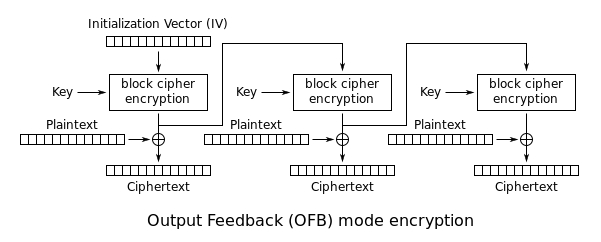
\includegraphics[width=\textwidth]{ofm.PNG}
\caption{Output Feedback Mode encryption}
\label{ofm}
\end{figure}

\subsubsection{CTR}

See Figure~\ref{ctr}.
Here, the nonce is the IV.

\begin{figure}
\centering
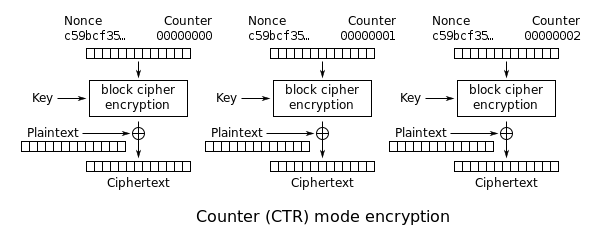
\includegraphics[width=\textwidth]{ctr.PNG}
\caption{CTR (counter) encryption}
\label{ctr}
\end{figure}

IV requirements:
\begin{itemize}
\item not secret
\item not random
\item don't reuse! (see OTP)
\end{itemize}

\subsection{FSR}

Stream cipher, designed for hardware.

\textbf{Algorithm}: we use a register of $n$ bits, $s_0, \dots, s_{n-1}$.
On one clock tick, $s_0$ is output, all registers shift one to the left, and $s_{n-1} = ff(s_0, \dots, s_{n-1})$, where $ff$ is the \textit{feedback function}.

\textbf{Example}
Key is an intitial state, $s_0, s_1, s_2, s_3$.
Key length is $n$.
\[
ff(s_0, s_1, s_2, s_3) = s_0 + s_1 \cdot s_2 + s_3.
\]
Example key is $1010$.
See Table~\ref{exFSR}.

\begin{table}
\centering
\begin{tabular}{c|c|c}
output & state & ff \\ \hline
& 1010 &0 \\
1 & 0100 & 1 \\
0 & 1001 & 1 \\
1 & 0011 & 0 \\
0 & 0110 & 0 \\
0 & 1100 & 0 \\
1 & 1000 & 0 \\
1 & 0000 & 1 \\
0 & 0001 & 0 \\
0 & 0010 & 1 \\
0 & 0101 & 0 \\
0 & 1010 & \\
\end{tabular}
\caption{Example FSR}
\caption{exFSR}
\end{table}
Note that this initial state has a period of 11.
We have not had all possible states yet.
5 left, see Table~\ref{exFSR2}.

\begin{table}
\centering
\begin{tabular}{c|c|c}
output & state & ff \\ \hline
& 1111 & 0 \\
1 & 1110 & 1 \\
1 & 1101 & 1 \\
1 & 1011 & 1 \\
1 & 0111 & 1 \\
0 & 1111 &
\end{tabular}
\caption{Example 2 of FSR}
\caption{exFSR2}
\end{table}

\begin{definition}[Periodic]
Let $(s_i)_{i=0}^{\infty}$ be a sequence.
$(s_i)$ is periodic if
\[
\exists r > 0 : s_{i+r} = s_i \forall i > 0
\]
If $r$ is minimal, then $r$ is called the \textit{period}, and $s_0, \dots, s_{r-1}$ is also called the \textit{period}.
\end{definition}

\begin{definition}[Ultimately periodic]
$(s_i)$ is called ultimately periodic if
\[
\exists r > 0, i_0 > 0 : s_{i+r} = s_{i} \forall i \ge i_0
\]
If both $r, i_0$ minimal, then $s_0, \dots, s_{i_0 - 1}$ is called the \textit{pre-period} and $s_{i_0}, \dots, s_{i_0 + r-1}$ is called \textit{period}.
\end{definition}

\begin{theorem}
Any outputs stream of FSR on $n$ bits is (ultimately) periodic with period $\le 2^n$.
\end{theorem}
\begin{proof}
After $2^{n}+1$ states, there are at least two equal states.
So, the period is in between those states.
\end{proof}

\textbf{Observation} either output stream is periodic or there is at least one state with at least two predecessors.

\begin{theorem}
If $(s_i)$ has period $r$ and for some $l > 0$ geldt $s_{i+l} = s_i \forall i \ge i_0$ for some $i_0$ then $r | l$, i.e. $l$ is a multiple of $r$.
\end{theorem}
\begin{proof}
$l = t \cdot r + r_0$, where $0 \le r_0 < r$.
Forall i big enough:
\begin{align*}
s_i &= s_{i+l} \\
&= s_{i+tr + r_0} \\
&= s_{i + (t-1)r + r_o} \\
&= \dots \\
&= s_{i+r_0}
\end{align*}

Then r is minimal, but $r_0$ is smaller, so $r_0 = 0$.
\end{proof}

\subsection{LFSR}

%TODO:
(zie schrift )

\subsubsection{Linear shift register}
Take:
\[
\ul{s}_0 = (s_0, \dots, s_{n-1}), \quad \ul{s}_1 = (s_1, \cdot, s_{n})
\]
with
\[
s_n = \sum_{i=0}^{n-1} c_i s_i
\]
Matrix C such that
\[
\ul{s}_i = \ul{s}_{i-1} \cdot C
\]
Take C
\[
C = \begin{pmatrix}
0 & 0 & \dots & 0 & c_0 \\
1 & 0 & \dots & & c_1 \\
\vdots & & & & \vdots \\
0 & & \dots & 1 & c_{n-1} \\
\end{pmatrix}
\]
Assume $c_0 = 1$.
\[
\det(C) = \pm 1
\]
so $C$ is invertible.

For a state $\ul{s_0}$, sequence $\ul{s}_{0}, \ul{s_1}, \dots$ becomes periodic, period is $r$.
\begin{align*}
\ul{s}_r &= \ul{s}_0 \\
\ul{s}_r &= \ul{s}_0 \cdot C^r \\
\end{align*}
True for all states:
\[
C^r = I
\]
and $r$ is smallest exp. $e > 0$ such that $C^e = I$.
Any possible period is devisor of $r$.

\begin{definition}
The \emph{order} of matrix $C$ is the smallest possible $r$ such that $C^r = I$.
\end{definition}

\subsubsection{Polynomials}

We have two functions:
\[
ff(t_0, \dots, t_{n-1}) = \sum_{i = 0}^{n-1} c_i t_i
\]
feedback function, and characteristic polynomial:
\[
cp(X) = X^n + ff(1, X, X^2, \dots, X^{n-1}) = X^n + \sum_{i = 0}^{n-1} c_i X^i
\]

\emph{degree} $n$ polynomial that lives in space $\mathbb{F}_2[X]$ (coefficients are of base 2).

\textbf*{Roots}

Root might be in exptension fields of $\mathbb{F}_2[X]$.
Take $\alpha$ as root of $cp(X)$.
Then we can take
\[
\alpha = X \mod cp(X).
\]
If $cp(X)$ is irreducible over $\mathbb{F}_2[X]$ (it does not factor over $\mathbb{F}_2[X]$), maybe this $X$ will even generate $\mathbb{F}_2[X] / cp(x)$.
If this is true, then the order is $2^{n-1}$, which is exactly what we want for LFSR.

Note:
\[
(1, \alpha, \alpha^2, \dots, \alpha^{n-1}) \cdot C = \left(\alpha, \alpha^2, \dots, \alpha^{n-1},  \sum_{i=0}^{n-1} c_i \alpha^i \right)
\]
This last term is equal to $\alpha^n$, because $\alpha$ is the root of the polynomial.
It could also be $- \alpha^n$, but we are working in $\mathbb{F}_2[X]$.
Which means
\[
\left(\alpha, \alpha^2, \dots, \alpha^{n-1}, \sum_{i=0}^{n-1}  c_i \alpha_i \right) = \alpha \cdot (0, \alpha, \dots, \alpha^{n-1}, \alpha^n)
\]
So $\alpha$ is an eigenvalue for $C$ and eigenvector for $\alpha$ is $(1, \alpha, \alpha^2), \dots, \alpha^{n-1}$.

\textbf*{Computing characteristic polynomial}

Compute characteristic polynomial in the eigen-theory sense, is going to be
\[
\det(C - \lambda I)
\]
We are working in $\mathbb{F}_2[X]$, which means minus is plus, so remove the minusses on the diagonal.
Now
\[
\det(C - \lambda I) = \lambda \cdot \begin{pmatrix}
\lambda & & & c_1 \\
1 & \ddots & & c_2 \\
& &  \lambda& \vdots \\
& & 1& c_{n-1} + \lambda \\
\end{pmatrix} + c_0 \cdot \begin{pmatrix}
1 & \lambda & & & \\
& 1 & \lambda & &  \\
& & \ddots & &  \\
& & & &\lambda  \\
& & & & 1 \\
\end{pmatrix}
\]
\begin{align*}
\det(C - \lambda I) &= \lambda \cdot \begin{pmatrix}
\lambda & & & c_1 \\
1 & \ddots & & c_2 \\
& &  \lambda& \vdots \\
& & 1& c_{n-1} + \lambda \\
\end{pmatrix} + c_0 \cdot \begin{pmatrix}
1 & \lambda & & & \\
& 1 & \lambda & &  \\
& & \ddots & &  \\
& & & &\lambda  \\
& & & & 1 \\
\end{pmatrix} \\
&= \lambda (\lambda \cdot (\lambda \dots \lambda (c_{n-1} + \lambda)) + c_1) + c_0 \\
&= c_0 + c_1 \lambda + c_2 \lambda^2 + \dots + c_{n-1} \lambda_{n-1} + \lambda^n \\
&= cp(X)
\end{align*}

\textbf*{Example}

\[
cp(X) = 1 + X + X^4
\]
This is irreducible over $\mathbb{F}_2[X]$:
\begin{itemize}
\item no zeros ($cp(0) = 1$, $cp(1) = 1$)
\item degree 2 factors: we are working in $\mathbb{F}_2[X]$, which means they should be of the form
\[
(X^2 + aX + 1)(X^2 + bX + 1) = X^4 + (a+b) X^3 + (1 + ab + 1)X^2 + (a+b)X + 1
\]
So $a+b = 0$, but also $a + b = 1$, which cannot become true.
So no degree 2 factors either.
\end{itemize}

Take $\alpha$ root of $1 + X + X^4$, so:
\[
\alpha^4 = \alpha + 1.
\]

We compute powers of alpha,
\[
1, \alpha, alpha^2, \alpha^3, \alpha^4 = \alpha + 1, \dots, \alpha^8 = \alpha^4 + \alpha^2 + \alpha = \alpha^2 + 1, \dots, \alpha^{15} = \alpha^4 + \alpha = 1
\]
What we did here, is exactly the same as the sequences (linear shift register) we used for feedback ciph register.
We see the state as the sequence of the coefficients of the polynomial and doing this computation is the same as doing LFSR.

Period maximal $2^{n-1} = 15$ has to do with fact that $\alpha$ is generator in $\mathbb{F}_2[X] / cp(X)$.

\textbf{Example 2}

\[
cp(X) = X^2 + X + 1
\]
degree $2$, so the LFSR has only two bits.
The polynomials that are not the highest degree give the constants for the shift registers (1 and 1).
\[
C = \begin{pmatrix}
0 & 1 \\
1 & 1
\end{pmatrix}
\]
Now:
\[
C^2 = \begin{pmatrix}
0 & 1 \\
1 & 1
\end{pmatrix} \cdot \begin{pmatrix}
0 & 1 \\
1 & 1
\end{pmatrix} = \begin{pmatrix}
1 & 1 \\
1 & 0
\end{pmatrix}
\]
Similarly:
\[
C^3 = \begin{pmatrix}
1 & 0 \\
0 & 1
\end{pmatrix} = I
\]
This is the identity matrix, so now it starts repeating.
So the order of $C$ is 3, which means this LFSR has only periods that are devisors of three.
Now, cp(X) is irreducible, and now the order implies that the order of cp(X) = 3.

\begin{definition}
$ord(cp(X))$ is smallest positive $e$ such that $X^e = 1 (\mod cp(X))$.
\end{definition}
As we did with the powers of $\alpha$ in example 1.

Example continued:

Let root of $cp(X)$ be $\tau$.
Let other root be $\bar{\tau}$.
Means:
\[
X^2 + X + 1 = (X - \tau)(X + \bar{\tau})
\]
Minus is plus:
\[
\tau + \bar{\tau} = 1, \quad \tau \cdot \bar{\tau} = 1
\]
Compute powers:
\[
1, \tau, \tau^2 = \tau + 1 = \bar{\tau}, \tau^3 = \tau \bar{\tau} = 1.
\]
This should not surprise you, since we we found this before.

\begin{theorem}
ord(cp(X)) = ord(C).
\end{theorem}

What does this tell us about LFRS? If we start in $10$, next will be $01$, then $11$, then back to $10$.

This is kind of like the Fibonachi sequence, but now in $\mathbb{F}_2[X]$.

\subsubsection{Theorems and definitions}

\begin{theorem}
Maximal period of LFSR with irreducible $cp(X)$ is equal to $ord(cp(X))$ as defined above.
\end{theorem}
\begin{proof}
Assume $s_{i+l} = s_l$ for all $i \ge 0$, but $l < ord(cp(X))$.
Then $l$ is not a maximal period.
Then $C^l \ne I$.
Take $\ul{s}_0 = (0, 0, \dots, 0, 1)$.
Now: $\ul{s}_1 = (0, \dots, 0, 1, *)$.
Now:
\[
s = \begin{pmatrix}
\emptyset & & 1 \\
& \dots &  \\
1 & & *  \\
\end{pmatrix}
\]
So:
\[
S \cdot C^l = S
\]
All its rows are independent, so $S$ is invertible:
\[
C^l = I
\]
Which leads to a contradiction.
\end{proof}

\begin{definition}
If $P(X)$ of degree $n$ over $\mathbb{F}_2$ is irreducible and it has order $2^{n-1}$ (in other words, the order of a root in $\mathbb{F}_{2^n}$ is $2^{n-1}$; in yet other words: any root of $P$ is generator of $\mathbb{F}_{2^n}^*$) then we say $P(X)$ is primitive polynomial.
\end{definition}
\begin{definition}
An LFSR has period $2^{n-1}$ iff its $cp(X)$ is primitive polynomial.
\end{definition}

Note: $\mathbb{F}_{2^n}^*$ is cyclic, so take some generator $g$.
It has minimal polynomial $P \in \mathbb{F}_{2}[X]$, degree $n$, $P(g) = 0$.
\[
\mathbb{F}_{2^n}^* = \{1, g, g^2, \dots, g^{2^{n-1}}, \quad ord(g) = 2^{n-1}
\]
Take LFSR with $cp(X)$ as such a $P$

Number of primitive polynomials = $\frac{\text{nr of primitive elt's }}{...} = \frac
{\phi(2^n-1)}{n}$.
This tells you there are lots and lots of primitive polynomials.

How do you find one?
Pick one, test if it is primitive, no?
Take another one.

\subsubsection{Golomb's criteria}
How does LFSR comply to Golomb?
(compare to case for $n=3$ to understand this)
Assume we have a period of length $2^{n}-1$ coming from LFSR with $n$ bits.
This means in the period (output of $ff$ of LFSR)every nonzero state occurs exactly once.
Count zeroes: $2^n$, states $n$ colums, half of them are zeroes, $-n$ because the all zero state is not actually there:
\[
n \cdot 2^n \cdot \frac{1}{2} - n = n(2^{n-1} - 1)
\]
Number of ones:
\[
n \cdot 2^{n-1}
\]
Colums in table are shifted periods: number of zeros in one period is $2^{n-1}-1$ and number of ones in one period is $2^{n-1}$.
So on the first criterium, we are doing excellent.

Second: similar argument.

Third Golomb: this is a problem... we have periodicity...
Compute autocorrelation, but not for period $2^{n}-1$ itself.

\begin{theorem}
$AC(k) = \begin{cases}
1 &\text{ if } 2^n - 1 | k \\
\frac{-1}{2^n - 1} &\text{ otherwise}
\end{cases}$
\end{theorem}

LFSR with a period of $2^{n}-1$ gives perfect colomb randomness within one period.

So: use LFSR to generate long key, as long as $2^n - 1$, use characteristic polynomial to find register coefficients.

\subsubsection{Adding characteristic polynomials}

\begin{theorem}
If $(s_i)$ has characteristic polynomial $cp^{(s)}(X)$ and $(t_i)$ has characteristic polynomial $cp^{(t)}(X)$.
Then $(s_i + t_i)$ as characteristic polynomial $lmc(cp^{(s)}(X), cp^{(t)}(X))$.
\end{theorem}

\textbf{Example}
\[
Cp(X) = X^5 + X^4 + 1 = (X^2 + X + 1)(X^3 + X + 1)
\]
Feedback polynomial:
\[
ff(s_0, \dots, s_4) = s_0 + s_4
\]
Check yourself that period is $21$ if we start with state $00001$.
Another period $7$ if we start at $00101$.
Period $3$ if we start at $01101$.

This is indication that the polynomial probably factors, since $7 = 2^3 - 1$, and $3 = 2^2 - 1$.
Not always true, but an indication!

If we look at the computation of the sequence starting with $00101$, we see that $s_3$ and $s_4$ depend on the first three bits, which means we could have used a smaller cp $X^3 + X + 1$ to generate this LFSR.
This is typical for factorizable LFSR cp.

Check the theorem:
As $s_i$, take the output of stream with period $3$
\[
s_i = 011 011 011 011
\]
and as $t_i$ the one with period $7$
\[
t_i = 001011100101110010111
\]
and so:
\[
s_i + t_i = 0100001111101010011001
\]
which is the output stream of the stream with period $21$.
There is structure in LFSR, which is bad in crypto.


\subsubsection{Problems with LFSR}

\begin{itemize}
\item If you know characteristic polynomial and $n$ successive states this enables you to "roll back".
If you know $C$, you can apply the inverse to compute predecessors.
\item If you don't know the characteristic polynomial and $2n$ states, then you can recover the characteristic polynomial. %TODO: huh?
\item If you even don't know $n$, you can simply guess it, then take $2n$ state, recover the candidate characteristic polynomial, check with next from states.
\end{itemize}
If you have enough output of the key stream, then you can break it!

\newpage
\section{NLFSR}

Non linear, they will be ultimately periodic, say of length $N$.
Then this period will be also generated by LFSR, namely with characteristic polynomial $X^n + 1$.
This is a very stupid LFSR: only the first register $s_0$ generates the output.
Now we know, every non-linear FSR will eventually become a linear one.

\begin{definition}
Linear complexity of NLFSR is smallest degree of characteristic polynomial of an LFSR that generates the period.
\end{definition}

Design goal for NLFSR's:
\begin{itemize}
\item get linear complexity high
\item get preperiods long
\end{itemize}
These are kind of conflicting...

\subsection{Grain}
See figure~\ref{grain}.

\begin{figure}[h!]
\centering
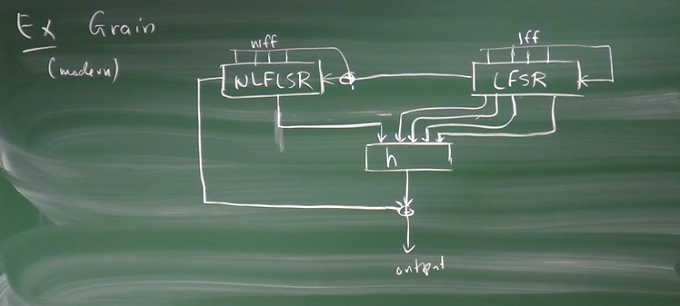
\includegraphics[width=\textwidth]{grain.PNG}
\caption{Grain NLFSR}
\label{grain}
\end{figure}

\subsection{AS/1}
Has to do with the \emph{kerkhof's principle}: if you design a cryptographic system, assume the enemy knows your algorithm.
Secrecy should only be in the key, not the algorithm.

\begin{figure}[h!]
\centering
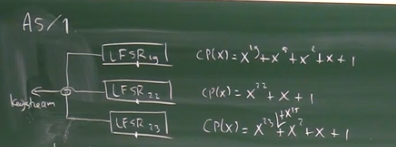
\includegraphics[width=\textwidth]{as1.PNG}
\caption{AS/1 NLFSR}
\label{as1}
\end{figure}

AS/1 was broken when the algorithm became known.
See figure~\ref{as1}.
Irregular clocking: bits 10 of $LFSR_{19}$, 11 of $LFSR_{22}$ and 12 of $LFSR_{23}$, take majority vote.
Clock only the LFSR's that match majority.

$64$-bit key and 32-bit IV, which is called the frame regular (114 bits = 1 frame).
Start with all-zero registers.
Add key bits to each register at last bit (instead of feedback) and every time you clock.
Do the same with IV bits.
In these steps totally disregard the output.
Then run for 100 steps without output.
Then output the key stream.

Crypto analysis: do brute force attack over $LFSR_{19}$ and $LFSR_{22}$, which has complexity $2^n$.
Then recover the initial state of $LFSR_{23}$.

\subsection{RC4}

Ron's Code, from L. R. Rivest.
Story is kind of similar unfortunately.

Byte-oriented.
    256-byte state, which always combines permutation of $0, 1, \dots, 255$.
    Key of $l$ bytes, $5 \le l \le 256$.
    5 bytes = 40 bits.

    RC4 setup: see figure~\ref{rc4}.

\begin{figure}[h!]
    \centering
    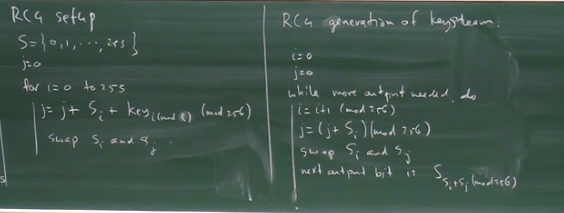
\includegraphics[width=\textwidth]{rc4.PNG}
    \caption{RC4 NLFSR}
    \label{rc4}
\end{figure}

    Analysis: second bytes has a bias towards being 0.
    If $s_2 = 0$ at the end of setup (happens with probability $\frac{1}{256}$).
    Then:


    If after setup $s_2 = 0$ then output second bit will be $0$, unless $2_1 = b = 2$.
    Second byte = 0 happens with probability $\frac{1}{256} \cdot \frac{255}{256} + \frac{255}{256} \cdot \frac{1}{256}$.
    This probability is twice as large as it should be.

    It gives you a byte-stream instead of a bit-stream.

\textbf{Analysis}

    Is used in WEP - Wired Equivalent Privacy.
    Password generates key, generates bytestream using RC4, generate bitstream from this, then use OTP on the bitstream and some message to get the ciphertext.

Now assume you are an attacker and you want to know the password.
    The password is unknown, but fixed, the IV is random but known.
    WEP always starts with the same message.
    RC4 bias: second keystream byte twice more likely to be zero.

    Start WEP protocol many times.
    With probability twice as large the second ciphertext byte = second plaintext byte.
    The first part of the message is always the same, and you do this many times, which means the ciphertext has the same bias as the key stream, and you can find the key bit causing the bias. (?)

    Other RC4 biases exist in first few keystream bytes: for example if first key byte fixed, then first keystream byte biased towards first key byte.

    Aircrack exploits these RC4 biases to break WEP.

    In exercises: play with this:
    \begin{itemize}
        \item write RC4 code
        \item write attack code
    \end{itemize}
    Needed are approximately $2^{18}$ RC4 encryptions to see effects.
    Preferably program in $C$.

    RC4 quick fix: throw away the first so may bytes.
\end{document}












